\documentclass[10pt,a4paper]{article}

\usepackage[utf8]{inputenc}
\usepackage{graphicx}

\usepackage[margin=19mm]{geometry}
\parskip 4.0pt  % Sets spacing between paragraphs.
% \renewcommand{\baselinestretch}{1.5}  % Uncomment for 1.5 spacing between lines.
\parindent 8.0pt  % Sets leading space for paragraphs.
\usepackage[font=sf]{caption} % Changes font of captions.

\usepackage{amsmath}
\usepackage{mathtools}
\usepackage{esint}
\usepackage{amssymb}
\usepackage{amsfonts}
\usepackage{multicol}
\usepackage{tabularx}
\usepackage{booktabs}
\usepackage{url} % Links
\usepackage[colorlinks=true, linkcolor=black, urlcolor=black, citecolor=black]{hyperref} % Links in words

\usepackage{subfiles}

\usepackage{listings}
\usepackage{xcolor}



\definecolor{codegreen}{rgb}{0,0.6,0}
\definecolor{codegray}{rgb}{0.5,0.5,0.5}
\definecolor{codepurple}{rgb}{0.58,0,0.82}
\definecolor{backcolour}{rgb}{0.95,0.95,0.92}

\lstdefinestyle{codecolour}{
    backgroundcolor=\color{backcolour},   
    commentstyle=\color{codegreen},
    keywordstyle=\color{magenta},
    numberstyle=\tiny\color{codegray},
    stringstyle=\color{codepurple},
    basicstyle=\ttfamily\footnotesize,
    breakatwhitespace=false,         
    breaklines=true,                 
    captionpos=b,                    
    keepspaces=true,                 
    numbers=left,                    
    numbersep=5pt,                  
    showspaces=false,                
    showstringspaces=false,
    showtabs=false,                  
    tabsize=2
}

% \lstset{style=mystyle, language= C++}

\title{Relazione Progetto Boids}
\author{Francesco Bartoli}
\date{}

\begin{document}

\maketitle

\tableofcontents

\setlength{\parindent}{0pt}


\section{Introduzione}
\subsection{Scopo}
Il programma ha come obiettivo quello di simulare in uno spazio bidimensionale il comportamento di stormi di uccelli in volo, che verranno indicati con il nome di \textit{boids}. 

\subsection{Installazione}

Le istruzioni su come compilare, testare, eseguire sono presentate nel README del progetto, riportato qui sotto:

\par\noindent\rule{\textwidth}{0.4pt}

Build instructions are for \textbf{Ubuntu 22.04}.

\subsubsection{Prerequisites}

\href{https://github.com/SFML/SFML}{SFML} (2.5): Library for graphic representation. \\
\href{https://github.com/texus/TGUI}{TGUI} (1.0): Library for graphic interface.

\subsubsection{SFML and TGUI Installation}

Install SFML:

\begin{lstlisting}
sudo apt-get install libsfml-dev
\end{lstlisting}

Install TGUI:

\begin{lstlisting}
sudo add-apt-repository ppa:texus/tgui
sudo apt update
sudo apt install libtgui-1.0-dev
\end{lstlisting}

\subsubsection{Clone the Repository}

\begin{lstlisting}[language=bash]
git clone https://github.com/Evyal/boids.git
\end{lstlisting}

\subsubsection{Build the Project}

\begin{itemize}
    \item \title{\textbf{Create the build directory}}

\begin{lstlisting}[language=bash]
mkdir build
cd build
\end{lstlisting}

\item \title{\textbf{Configure CMake in Release mode}}

\begin{lstlisting}[language=bash]
cmake .. -DCMAKE_BUILD_TYPE=Release
\end{lstlisting}

\item \title{\textbf{Build the project}} 

\begin{lstlisting}[language=bash]
cmake --build .
\end{lstlisting}
\end{itemize}


\subsubsection{Running the program} 

\begin{lstlisting}[language=bash]
./boids
\end{lstlisting}

\par\noindent\rule{\textwidth}{0.4pt}

\newpage

\section{Struttura del programma}
Segue una breve descrizione delle principali scelte progettuali e implementative del programma.


I file del progetto sono organizzati in sottocartelle, nello specifico i \texttt{.cpp} si trovano nella \texttt{/source}, mentre i rispettivi header sono situati nella \texttt{/include}. La directory \texttt{/testing} contiene i file di testing, e infine in \texttt{/assets} sono presenti alcuni file necessari per il corretto funzionamento del programma. 

\subsection{Regole di volo}

I \textit{boids} si seguono delle regole di volo, che ne determinano il comportamento. Ad ogni istante, il programma modifica le velocità e le posizioni dei \textit{boids} attraverso le seguenti formule:

\begin{equation*}
    \vec{v}_{bi} = \vec{v}_{bi} + \vec{v}_S + \vec{v}_A + \vec{v}_C + \vec{v}_R
\end{equation*}

\begin{equation*}
    \vec{x}_{bi} = \vec{x}_{bi} + \vec{v}_{bi} \Delta t
\end{equation*}

Dove $\vec{v}_S$, $\vec{v}_A$, $\vec{v}_C$, e $\vec{v}_R$ sono rispettivamente:

\subsubsection{Separazione}

\begin{equation*}
    \vec{v}_S = -s \sum_{j \neq i} (\vec{x}_{b_j} - \vec{x}_{b_i}) \quad \text{se} \quad \left| \vec{x}_{b_i} - \vec{x}_{b_j} \right| < d_s
\end{equation*}

\subsubsection{Allineamento}

\begin{equation*}
    \vec{v}_A = a \left( \frac{1}{n-1} \sum_{j \neq i} \vec{v}_{b_j} - \vec{v}_{b_i} \right) \quad \text{se} \quad \left| \vec{x}_{b_i} - \vec{x}_{b_j} \right| < i
\end{equation*}

\subsubsection{Coesione}

\begin{equation*}
    \vec{x}_c = \frac{1}{n-1} \sum_{j \neq i} \vec{x}_{b_j} \quad \text{se} \quad \left| \vec{x}_{b_i} - \vec{x}_{b_j} \right| < i
\end{equation*}

\begin{equation*}
    \vec{v}_C = c (\vec{x}_{c} - \vec{x}_{b_j})
\end{equation*}

Dove $n-1$ assume valori dipendenti dal numero di boid nel range di interazione, e non è un valore fisso dipendente dal numero di boids nello stormo.

E $s, ds, a, c, i$ sono parametri della simulazione, e nel progetto sono indicati con i nomi di \textit{separationStrength}, \textit{separationRange}, \textit{alignmentStrength}, \textit{cohesionStrength} e \textit{interactionRange}.

\subsubsection{Repulsione}

Questa regola in termini di formula è analoga a quella della separazione e determina l'allontanamento tra \textit{boids} di stormi differenti introducendo due nuovi parametri $r, dr$, che nel progetto sono indicati con i nomi di \textit{repelStrength} e \textit{repelRange}.

\subsubsection{Interazione \textit{On Click}}

\begin{equation*}
    \vec{v} = \pm p \sum_{j} (\vec{x}_{b_j} - \vec{x}) \quad \text{se} \quad \left| \vec{x}_{b_j} - \vec{x} \right| < i
\end{equation*}

Anche questa regola ha una formula analoga a quella della separazione e permette all'utente di interagire con i boids. Il $\pm$ è dovuto al fatto che questa interazione può essere sia attrattiva che repulsiva mentre $\vec{x}$ è il punto in cui l'utente ha cliccato. Il parametro che determina l'intensità di questa interazione prende il nome di \textit{clickStrength} all'interno del progetto.

\newpage

\subsection{Files}

Tutti i file del progetto sono stati inseriti nel namespace \texttt{ev}. Tutti i file menzionati di seguito come \texttt{.cpp} hanno un corrispettivo header.

\subsubsection{constants.hpp}

Namespace che contiene valori come limiti di velocità o posizione per i \textit{boids}, parametri di interazione di default, o ulteriori valori per l'inizializzazione degli elementi dell'interfaccia grafica.

\subsubsection{structs.hpp}

Struct per impacchettare dei valori usati per inizializzare bottoni o altri elementi di interfaccia grafica

\subsubsection{boid.cpp}

File di implementazione della classe Boid e funzioni ausiliare per gestirne il comportamento

\subsubsection{flock.cpp}

File di implementazione della classe Flock che determina la struttura collettiva dei \textit{boids} all'interno di uno stormo.

\subsubsection{random.cpp}

File che si occupa della generazione di numeri casuali

\subsubsection{statistics.cpp}

File che si occupa del calcolo delle statistiche restituite a schermo, riguardanti valori medi e deviazioni standard delle posizioni e velocità dei \textit{boids}.

\subsubsection{graphics.cpp}

Breve file che contiene una funzione per la corretta rappresentazione grafica dei \textit{boids}, ed un'altra che costruisce un rettangolo (\texttt{sf::Rectangle}) prendendo come parametro una delle struct definita nel file sopracitato.

\subsubsection{switchbutton.cpp}

La classe Switchbutton introduce la funzionalità di un bottone che può trovarsi in due stati, non fornita da TGUI.

\subsubsection{gui.cpp}

Classe che introduce gli elementi necessari a costruire l'interfaccia grafica del programma, e si occupa di coordinare tutti i file che implementano la logica all'interno di essa. 

\newpage

\section{Interfaccia della simulazione}
%descrizione del formato di input e di output, possibilmente con degli esempi

Anche questa parte deriva in parte dal README del progetto.

\begin{center}
    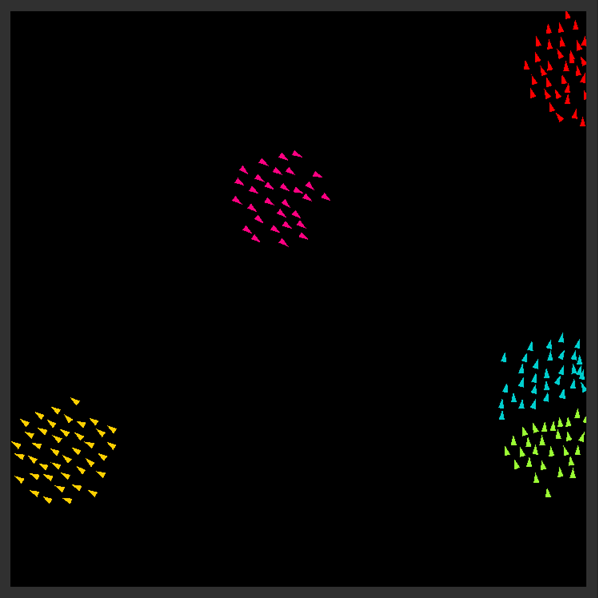
\includegraphics[width=1.0\textwidth]{../images/interface.png}
\end{center}

\maketitle{\textbf{Features}}

- Real-time visualization of flock movement \\
- Real-time statistics display for each flock \\
- Interactive controls for adding or removing flocks \\
- Adjustable parameters for interactions between boids \\

\begin{center}
    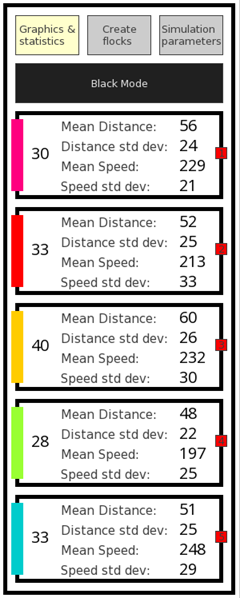
\includegraphics[width=0.32\textwidth]{../images/option1.png}
    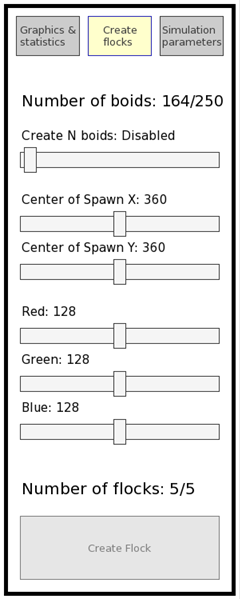
\includegraphics[width=0.32\textwidth]{../images/option2.png}
    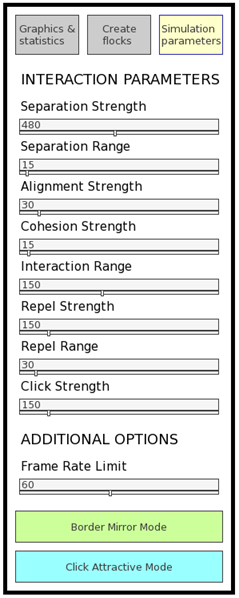
\includegraphics[width=0.32\textwidth]{../images/option3.png}
\end{center}


\subsection{Option 1: Graphics and statistics} 

- \textbf{Background color button}: Changes the colour of the background. (black and white) \\
- \textbf{Red numbered buttons}: Delete the corresponding flock.

\subsection{Option 2: Create Flocks}

- \textbf{Number of boids slider}: Selects the number of boids for a new flock. \\
- \textbf{Center of spawn sliders}: Select the spawn location of a new flock. \\
- \textbf{RGB sliders}: Select the color of a new flock. (Creating a white or black flock is disallowed because it would be invisible) \\
- \textbf{Create flock button}: Creates a new flock if there is enough space. (Max 250 boids; Max 5 flocks)

\subsection{Option 3: Simulation Parameters}

- \textbf{Interaction parameters sliders}: Change the values of the parameters of the rules that determine the movement of \textit{boids}. \\
- \textbf{Border mode button}: Changes the behaviour of \textit{boids} at the borders. (mirror or toroidal) \\
- \textbf{Click mode button}: Changes the interaction on click. (attractive or repulsive)

\subsection{Key Controls}

- \textbf{Left Click}: Interact with boids, attracting or repelling them to cursor. \\
- \textbf{Space Bar}: Pause/Resume simulation.

\newpage

\section{Testing}
%strategia di test per verificare che quanto ottenuto sia ragionevolmente esente da errori

Tutti i file incaricati dell'implementazione di parte della logica del programma hanno un corrispettivo file di testing. Più precisamente, sono presenti i seguenti: \texttt{testboid.cpp}, \texttt{testflock.cpp}, \texttt{testrandom.cpp} e \texttt{teststatistics.cpp}. 

Attraverso i test si è cercato di controllare che le classi, i metodi delle classi e le funzioni introdotte fossero esenti da errori e mostrassero il comportamento atteso. Sono stati eseguiti test in casi semplici per poter stabilire il funzionamento corretto del codice, e anche in alcuni casi particolari quando ritenuto necessario.

Il framework che si è utilizzato per creare le testing unit è doctest.h, il cui file è incluso nella cartella nel progetto (\texttt{/assets/doctest.h}). Questa libreria è in grado di generare autonomamente un main e permette l'esecuzione dei test semplicemente includendo il file sopracitato.

\subsection{Eseguire i test}

Per potere eseguire i test è necessario trovarsi nella cartella dove vengono prodotti gli eseguibili dei file precedentemente menzionati, seguendo i passaggi elencati sotto. Immaginando di trovarsi nella cartella principale dov'è contenuto il progetto:

\begin{lstlisting}[language=bash]
    cd build
    cd testing
\end{lstlisting}

E digitare il comando corrispondente al test che si vuole eseguire: 

\begin{lstlisting}[language=bash]
    ./testboid
    ./testflock
    ./testrandom
    ./teststatistics
\end{lstlisting}

O eventualmente eseguendoli tutti in una volta utilizzando il seguente comando

\begin{lstlisting}[language=bash]
    ctest
\end{lstlisting}


\section{Descrizione dei risultati}
%interpretazione dei risultati ottenuti


\section{Links}

\setlength{\parindent}{20pt}
Link alla repository di github utilizzata durante la realizzazione del progetto.

\url{https://github.com/Evyal/boids}


\end{document}